% !TEX TS-program = pdflatex
% !TEX encoding = UTF-8 Unicode

% This is a simple template for a LaTeX document using the "article" class.
% See "book", "report", "letter" for other types of document.

\documentclass[11pt]{article} % use larger type; default would be 10pt

\usepackage[utf8]{inputenc} % set input encoding (not needed with XeLaTeX)

%%% Examples of Article customizations
% These packages are optional, depending whether you want the features they provide.
% See the LaTeX Companion or other references for full information.

%%% PAGE DIMENSIONS
\usepackage
[a4paper,bindingoffset=0.2in,%
 left=1.75in,right=1.75in,top=2in,bottom=2in,%
 footskip=.25in]
{geometry} % to change the page dimensions
%\geometry{a4paper} % or letterpaper (US) or a5paper or....
% \geometry{margin=2in} % for example, change the margins to 2 inches all round
% \geometry{landscape} % set up the page for landscape
%   read geometry.pdf for detailed page layout information

\usepackage{graphicx} % support the \includegraphics command and options

% \usepackage[parfill]{parskip} % Activate to begin paragraphs with an empty line rather than an indent

%%% PACKAGES
\usepackage{booktabs} % for much better looking tables
\usepackage{array} % for better arrays (eg matrices) in maths
\usepackage{paralist} % very flexible & customisable lists (eg. enumerate/itemize, etc.)
\usepackage{verbatim} % adds environment for commenting out blocks of text & for better verbatim
\usepackage{subfig} % make it possible to include more than one captioned figure/table in a single float
% These packages are all incorporated in the memoir class to one degree or another...

%%% HEADERS & FOOTERS
\usepackage{fancyhdr} % This should be set AFTER setting up the page geometry
\pagestyle{fancy} % options: empty , plain , fancy
\renewcommand{\headrulewidth}{0pt} % customise the layout...
\lhead{}\chead{}\rhead{}
\lfoot{}\cfoot{\thepage}\rfoot{}

%%% SECTION TITLE APPEARANCE
\usepackage{sectsty}
\allsectionsfont{\sffamily\mdseries\upshape} % (See the fntguide.pdf for font help)
% (This matches ConTeXt defaults)

%%% ToC (table of contents) APPEARANCE
\usepackage[nottoc,notlof,notlot]{tocbibind} % Put the bibliography in the ToC
\usepackage[titles,subfigure]{tocloft} % Alter the style of the Table of Contents
\renewcommand{\cftsecfont}{\rmfamily\mdseries\upshape}
\renewcommand{\cftsecpagefont}{\rmfamily\mdseries\upshape} % No bold!

%%% END Article customizations

%%% The "real" document content comes below...

\usepackage{tabulary}
\usepackage{pgfgantt}
\usepackage{pdflscape}
\usepackage{enumitem}
\usepackage{pdfpages}

\definecolor{textblack}{RGB}{0, 25, 50}
\definecolor{backgroundwhite}{RGB}{240,250,255}

\linespread{1.2}

\newcommand{\AnalisiSituazioneAttualeTabella}[5]{
	\begin{tabular}[c]{|m{1in}|m{2.5in}|}
		\hline
		Settore & #1 \\ \hline
		Attività & #2 \\ \hline
		Situazione \\informativa & #3 \\ \hline
		Modalità \\operativa & #4 \\ \hline
		Obiettivo & #5 \\ \hline
	\end{tabular}
	\vspace{20pt}
}

\newcommand{\RequisitiSpecifici}[3]{
	\begin{description}[align=right,labelwidth=3cm]
		\item[Requisiti: ] #1
		\item[Attori: ] #2
		\item[Caso d'Uso: ] #3
	\end{description}
}

\newenvironment{requisiti}
{
	\newcommand{\requisito}[3]{
		##1 & ##2 & ##3 \\ \hline
	}
	%begin
	\tabulary{\textwidth}{|m{1in}|m{2in}|m{1.5in}|}
	\hline
	Requisiti & Settori & Caso d'Uso \\ \hline
}
{%end
	\endtabulary
	\vspace{20pt}
}

%\renewenvironment{requisiti}
%{ \rule{1ex}{1ex}\hspace{\stretch{1}} }
%{ \hspace{\stretch{1}}\rule{1ex}{1ex} }

%\setlength{\textwidth}{350pt}
%\setlength{\marginparwidth}{0pt}

\title{Fattibilità e Vision}
\author{Gabriele Giudici \& Simone Mosciatti}
%\date{} % Activate to display a given date or no date (if empty),
         % otherwise the current date is printed 

\begin{document}
\color{textblack}
\pagecolor{backgroundwhite}

\maketitle

\tableofcontents



\section{Obiettivi}

L'obbiettivo del nostro progetto è quello di migliorare il sistema informativo già esistente della piscina di Riccione apportando buove funzionalità al sistema.

L'intervento si concentrerà su:

\begin{enumerate}
	\item Gestione degli iscritti, automatizzando le procedure di rinnovo della quota associativa
	\item Gestione delle corsie della piscina, permettendo la prenotazione delle corsie in modo da evitare sovraffollamento
	\item Gestione degli eventi, automatizzando la procedura di affitto della intera struttura per eventi
	\item Cooperazione con ACQUALIS per mantenere bassi i costi di sviluppo della applicazione.
\end{enumerate}

L'applicattivo avrà funzionalità di sostegno ai reparti: Amministrazione Attività Sportive,  Gestione Finanze e Rapporti con Enti Esterni.



\section{Introduzione}


La piscina è utilizzata dagli atleti olimpici della Federazione Italiana Nuoto (FIN) durante gli ordinari allenamenti ed essendo una delle migliori in Italia è spesso luogo designato per ospitare varie manifestazioni.

Parte del costo del sistema informativo verrà abbattuto tramite una partership con ACQUALIS, nota società di distribuzione di prodotti relativi al nuoto.

La partership prevederà l'introduzione di uno store all'interno del portale web della piscina dedicato esclusivamente ai prodotti ACQUALIS.

Si vogliono introdurre diverse funzionalità:
\begin{enumerate}
	\item Semplice ed automatica gestione degli iscritti con automatico rinnovo delle quote via pagamento online. 
	\item Possibilità di prenotare corsie per gli allenamenti, sia da parte della FIN che da parte dei normali fruitori della piscina.
	\item Possibilità di prenotare l'intera struttura per manifestazioni ed eventi.
	\item Creazione di store online integrato di ACQUALIS.

\subsection*{Stackeholder}

\begin{itemize}
	\item Ente gestore della piscina
	\begin{itemize}
		\item Amministrazione Attività Sportive
		\item Gestione Finanze
		\item Rapporti con Enti Esterni
	\end{itemize}
	\item FIN
	\begin{itemize}
		\item Allenatori
		\item Atleti
		\item Personale organizzativo
	\end{itemize}
	\item Privati fruitori della piscina
	\item ACQUALIS
\end{itemize}


\section{Background}

Il sistema informativo della piscina è limitato a pochi personal computer con semplice gestione di basi di dati da suite di automazione.

La maggior parte delle operazioni viene effettuata a mano in modo lento e ripetitivo dal personale di segreteria.


Il sistema è gia integrato con un centro medico della zona che gestisce le visite mediche degli atleti.


\end{enumerate}

\section{Analisi della situazione attuale}

La situazione attuale è la seguente:

\AnalisiSituazioneAttualeTabella
	{Amministrazione Attività Sportive}
	{Controlli sul regolare pagamento delle quote e relative scadenze}
	{Computer con suite di office automation}
	{Ad inizio settimana a tutti gli iscritti a cui scaderà la quota entro la fine della settimana viene mandata una email ricordando di pagare la quota di persona in piscina}
	{Rinnovo della quota di iscrizione con possibilità di pagamenti in via telematica}

\AnalisiSituazioneAttualeTabella
	{Amministrazione Attività Sportive e Rapporti con Enti Esterni}
	{Prenotazione dei turni per la fruizione delle corsie di allenamento}
	{Nessun sistema informatico.}
	{I bagnini decidono autonomamente come allocare le corsie bilanciando i vari bisogni del momento.}
	{Possibilità di prenotazione delle corsie in anticipo via web così da evitare il sovraffolamento della piscina e permettere alla FIN di allenarsi in modo consistente e continuo.}

\AnalisiSituazioneAttualeTabella
	{Rapporti con Enti Esterni}
	{Organizazione e supporto di grandi eventi}
	{Suite di office automation}
	{Tutti i contatti sono gestiti dal personale amministrativo che dopo una richiesta di prenotazione via email controlla che la data sia disponibile, in caso affermativo richiede il pagamento di una caparra e, a pagamento avvenuto, alloca la struttura per la data richiesta. Viene quindi affisso un cartello in bacheca indicando la data in cui tutta la struttura è prenotata e inagibili per i normali fruitori.}
	{Automatizzare il processo di prenotazione della struttura e invio automatico di comunicazione telematica ai soci della società per comunicare l'inagibilità nel giorno programmato.}

\AnalisiSituazioneAttualeTabella
	{Rapporti con Enti Esterni}
	{Parternship con ACQUALIS}
	{Nessuna, lo sviluppo del sistema informativo rappresenta l'inizio della collaborazione tra la società e ACQUALIS}
	{Nessuna}
	{Creare un store web-based dove i fruitori della piscina possono accedere ai prodotti offerti da ACQUALIS}

\section{Descrizione dei problemi}

I problemi riscontrati al momento sono:

\begin{itemize}
	\item Sovraffolamento della piscina con utenze concentrate in pochi particolari orari
	\item Conflitti tra i privati fruitori della piscina e la FIN per l'uso delle corsie di allenamento.
	\item Operazione amministrative svolte in modo lento, ripetitivo, prono ad errori e non integrato.
	\begin{itemize}
		\item Problemi di integrazione tra le manifestazioni e il normale utilizzo della piscina
		\item Lentezza nel riscuotere le quote associative
	\end{itemize}
\end{itemize}

\section{Soluzioni proposte}

Proponiamo lo sviluppo di applicativi web-based per:

\begin{itemize}
	\item Gestione rinnovo quote
	\item Possibilità di prenotazione di posti nelle corsie di allenamento
	\item Automatizzazione per la prenotazione della intera struttura
	\item Store ACQUALIS dedicato ai membri della piscina
\end{itemize}


Abbiamo individuato tre possibilità per implementare la soluzione proposta.

\begin{enumerate}
	\item Acquisto di un sistema completo ERP da fornitori esterni. Questa soluzione rende molto veloci i tempi di realizzazione del sistema ma è relativamente costosa, poco adattabile alle specifiche esigenze della società e lega molto la società al futuro del fornitore del sistema ERP.
	\item Implementazione completa del sistema. Questa soluzione lascia il maggior margine di manovra nella creazione del sistema informativo, i costi sono soltanto quelli di sviluppo del prodotto, ma i tempi sono decisamente lunghi.
	\item Implementazione del sistema basandosi su framework open source. Questa soluzione è un buon compromesso tra le due precedenti, usando tecnologia matura e già conosciuta è possibile tenere i tempi di sviluppo della applicazione relativamente bassi, in più -- usando framework open source -- i costi del sistema sono solo quelli relativi allo sviluppo e la società non si lega in modo troppo stretto a nessun fornitore.
\end{enumerate}

Consigliamo la terza opzione in quanto la più equilibrata che permette rapidi tempi di sviluppo, non impone vincoli rispetto alla creazione di particolari features e usando popolari framework rende possibile una facile manutenzione del sistema.

Sconsigliamo invece la prima opzione in quanto molto costosa, poco adattabile agli specifici bisogni della società ed in oltre legherebbe molto strettamente il sistema informativo al fornitore del ERP rendendo più costosa la manutenzione del sistema stesso.

Ci sentiamo anche di scongliare la seconda opzione in quanto allungherebbe i tempi di sviluppo senza portare particolari benefici alla società, in oltre, una implementazione completamente nuova di un sistema informativo renderebbe lenta e difficile la manutenzione del sistema in quanto solo gli sviluppatori della applicazione avrebbero una conoscenza sufficientemente dettagliata del sistema per poter intervenire in modo rapido ed economico.

\section{Driver (B)}

La adozione del sistema informativo è guidata da driver sia di efficacia che di efficienza.

\subsection{Efficacia}

\begin{description}
	\item[Rendere la piscina più organizzata e creare un servizio più fruibile che porterà ad un aumento di iscritti: ]La possibilità di prenotare posti e corsi di allenamento permette di evitare conflitti e malcontenti nel bordo vasca, oltre che permettere un più constante e continuo allenamento degli atleti della FIN
\end{description}
\subsection{Efficienza}

Molti features del Sistema Informativo migliorano l' efficienza della associazione.

\begin{description}
	\item[Automatica gestione del rinnovo delle quote:] la gestione informatizzata renderà molto più snello e veloce il lavoro del personale amministrativo, inoltre sarà possibile tenere meno soldi in cassa aumentando la sicurezza della struttura. 
	\item[Automatica prenotazione della intera struttura:] la gestione informatizzata eviterà che il pesonale continui a rispondere a richieste di persone poco interessate e permetterà di concentrare le risorse solo per gli enti che hanno già pagato la caparra e riuscendo a garantire un servizio migliore.
\end{description}

\section{Struttura dell' organizzazione (O)}

La società è relativamente piccola ed è divisa in pochi dipartimenti che comunica molto tra di loro in maniera informale.

La struttura della società è rappresentata nel seguente organigramma.

\vspace{0.75in}
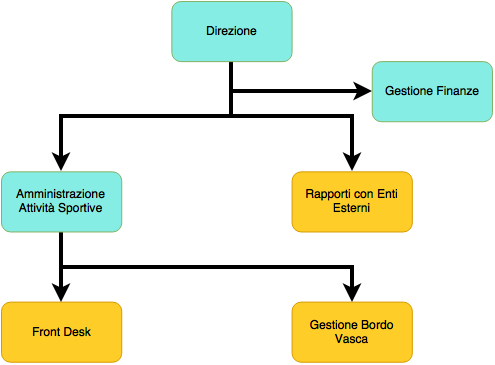
\includegraphics[scale=0.7]{Organigramma}
\vspace{0.75in}

Date le piccole dimensioni della società è chiaro che tutti i reparti saranno interessati, almeno indirettamente dal nuovo sistema informativo, i reparti direttamente interessati sono evidenziati in giallo.

\section{Requisiti funzionali}

\begin{enumerate}
	\item La società richiede periodicamente ai soci il rinnovo delle quote associative via email, i soci pagano online oppure alla segreteria.
	\item La società dispone di un portale web dove i fruitori della piscina devono prenotarsi per sfruttare le corsie.
	\item La società dispone di un portale web nel quale è possibile fare richiesta di prenotazione dell'intera struttura per un periodo di tempo limitato. Il responsabile riceverà una notifica e sarà suo compito mettersi in contatto con l'ente esterno.
	\item La società dispone di uno store online dedicato ad uso dei soci gestito da ACQUALIS
\end{enumerate}


\subsection{Requisiti funzionali Specifichi}

\begin{enumerate}
	\item La società richiede periodicamente ai soci il rinnovo delle quote associative via email, i soci pagano online oppure alla segreteria.
	\begin{enumerate}
		\item Ogni 24 ore uno script automatico ricerca tutti gli iscritti la cui quota è in scadenza e invia a questi una email invitanto a rinnovare la quota in via telematica o in sede
		\item Il servizio web della segreteria viene aggiornato in modo tale da evidenziare i soci che devono ancora pagare la quota
		\item Al pagamento della quota via online, il servizio web è automaticamente aggiornato per mostrare che il socio ha effettivamente rinnovato la quota
		\item Al pagamento della quota in sede, il personale può marcare che il socio ha rinnovato la propria quota.
	\end{enumerate}

	\item La società dispone di un portale web dove i fruitori della piscina devono prenotarsi per sfruttare le corsie.
	\begin{enumerate}
		\item La compilazione della richiesta è guidata dal sistema e permessa dopo autenticazione.
		\item I dati della prenotazione, previa verifica di disponibilità, sono automaticamente inseriti nel sistema
		\item Viene inviata una email per ricordare l'avvenuta prenotazione
		\item Personale autorizzato della società può consultare l'elenco delle prenotazioni per risolvere possibili equivoci a bordo vasca
	\end{enumerate}
	\item La società dispone di un portale web nel quale è possibile fare richiesta di prenotazione dell'intera struttura per un periodo di tempo limitato. Il responsabile riceverà una notifica e sarà suo compito mettersi in contatto con l'ente esterno.
	\begin{enumerate}
		\item Il prezzo e la disponibilità della struttura sono mostrati in un interfaccia web
		\item L'utente compila un questionario guidata dalla piattaforma
		\item Il sistema notifica al responsabile del reparto ``Rapporti con Enti Esterni'' l'avvenuta richiesta di prenotazione
	\end{enumerate}
	
	
	\item La società dispone di uno store online dedicato ad uso dei soci gestito da ACQUALIS
	\begin{enumerate}
		\item Lo store si interfaccia in via telematica alla piattaforma di ACQUALIS la quale comunica i prodotti da mostrare, i prezzi e le quantità disponibili
		\item All'acquisto di un prodotto il pagamento viene gestito completamente da ACQUALIS
		\item Dopo l'acquisito viene richiesto se si preferisce ricevere il prodotto a casa o direttamente in piscina, tale richiesta viene inoltrata ad ACQUALIS
		\item Nel caso in cui venga deciso di ricevere il prodotto in piscina, il personale viene avvertito e tiene in consegna il prodotto finchè il socio non lo richiede.
	\end{enumerate}
\end{enumerate}

\begin{requisiti}
	\requisito{Ricerca quote in scadenza}
			{Sistema Automatico}
			{Controllo Quote}
	\requisito{Aggiornamento Sistema Segreteria}
			{Sistema Automatico, Front Desk}
			{Aggiornamento interfaccia web}
	\requisito{Pagamento Quote Online}
			{Banca, Sistema Automatico, Soci Iscritti, Front Desk}
			{Pagamento Telematico}
	\requisito{Pagamento Quota In Sede}
			{Soci Iscritti, Front Desk}
			{Pagamento Manuale}
\end{requisiti}

\begin{requisiti}
	\requisito{Compilazione Prenotazione}
			{Soci Iscritti, Personale FIN}
			{Prenotazione Corsie}
	\requisito{Inserimento prenotazione nel sistema}
			{Sistema Automatico}
			{Allocazioe Corsie}
	\requisito{Comunicazione Avvenuto Prenotazione}
			{Sistema Automatico, Soci Iscritti, Personale FIN}
			{Conferma Prenotazione}
	\requisito{Consultazione Prenotazioni}
			{Personale Autorizzato}
			{Verifiche Prenotazioni}
\end{requisiti}

\begin{requisiti}
	\requisito{Visualizzazione Costi}
			{Utente Esterno, Sistema Automatico}
			{Visualizzazione Costi}
	\requisito{Compilazione Questionario}
			{Utente Esterno, Sistema Automatico}
			{Richiesta Noleggio Struttura}
	\requisito{Comunicazione con il responsabile}
			{Sistema Automatico, Responsabile del reparto ``Rapporti con Enti Esterni''}
			{Notifica Responsabile}
\end{requisiti}

\begin{requisiti}
	\requisito{Visualizzazione prodotti disponibili}
			{Sistema Automatico, Soci Iscritti, ACQUALIS}
			{Visualizzazione Prodotti}
	\requisito{Pagamento}
			{ACQUALIS, Soci Inscritti}
			{Pagamento}
	\requisito{Richiesta estremi spedizione}
			{ACQUALIS, Soci Inscritti, Sistema Automatico}
			{Estremi spedizione}
	\requisito{Ricezione spedizione in piscina}
			{Sistema Automatico, Personale, Soci Inscritti}
			{Ricezione spedizione in piscina}
\end{requisiti}

\section{Requisiti Non funzionali}

\begin{description}
	\item[Prestazioni] Supporto per 150 connesioni simultanee
	\item[Qualità dei dati] Dati aggiornati al completamento delle richieste
	\item[Efficienza] Massimo tempo di risposta ad ogni richiesta web 2sec, 90 percentile massimo a 0.5sec
	\item[Efficacia] Netto snellimento delle pratiche burocratiche, riduzione dei conflitti nel piano vasca, riduzione del sovraffolamento.
	\item[Robustezza] Possibile downtime programmato per manutenzione di massimo tre ore ogni 6 mesi, affidabilità con 0.999 \%
	\item[Sicurezza] Non memorizzazione di dati sensibile degli utenti, in particolare evitare la memorizzazione di numero, codice di sicurezza e data di scadenza delle carte di credito.
	\item[Disponibilità] Servizio consultabile 24/7/365
	\item[Usabilità] Usabilità da dispositivi mobile e fissi, massimo 6 click per raggiungere ogni funzione, massimo 2 click per raggiungere le 5 funzioni più usate. Compatibilità con i maggiori browser IE7, Chrome, Firefox, Opera.
\end{description}

%sicurezza, performace, usabilità

\section{Gantt}

\newganttlinktype{jumpOneConnectStart}{
	\ganttsetstartanchor{on bottom=0.5}
	\ganttsetendanchor{on left}
	\draw [/pgfgantt/link]
	% first segment (down)
	(\xLeft, \yUpper) --
	(\xLeft, \yUpper - \ganttvalueof{y unit chart} / 4) --
	(\xRight + \ganttvalueof{link bulge} * \ganttvalueof{x unit} * 5, 
		\yUpper - \ganttvalueof{y unit chart} / 4) --
	(\xRight + \ganttvalueof{link bulge} * \ganttvalueof{x unit} * 5, 
		\yUpper - \ganttvalueof{y unit chart} * 1.3) --
	(\xRight - \ganttvalueof{link bulge} * \ganttvalueof{x unit} * 2, 
		\yUpper - \ganttvalueof{y unit chart} * 1.3) --
	(\xRight - \ganttvalueof{link bulge} * \ganttvalueof{x unit} * 2, 
		\yLower) --
	(\xRight, \yLower);
}


\newganttlinktype{middleToStart}{
	\ganttsetstartanchor{on bottom=0.5}
	\ganttsetendanchor{on left}
	\draw [/pgfgantt/link]
	% first segment (down)
	(\xLeft, \yUpper) --
	(\xLeft, \yUpper - \ganttvalueof{y unit chart} / 4) --
%	(\xRight + \ganttvalueof{link bulge} * \ganttvalueof{x unit} * 5, 
%		\yUpper - \ganttvalueof{y unit chart} / 4) --
%	(\xRight + \ganttvalueof{link bulge} * \ganttvalueof{x unit} * 5, 
%		\yUpper - \ganttvalueof{y unit chart} * 1.3) --
	(\xRight - \ganttvalueof{link bulge} * \ganttvalueof{x unit} * 2, 
		\yUpper - \ganttvalueof{y unit chart} / 4) --
	(\xRight - \ganttvalueof{link bulge} * \ganttvalueof{x unit} * 2, 
		\yUpper - \ganttvalueof{y unit chart} * 1.3) --
	(\xRight - \ganttvalueof{link bulge} * \ganttvalueof{x unit} * 2, 
		\yLower) --
	(\xRight, \yLower);
}

% studio di fattibilità 11gg
% pianificazione 13gg
% identificazione e analisi requisiti 15gg
% definizione architettura 12gg
% implementazione 30gg
%definizione UI|UX 11gg
% implementazione UI|UX 30gg
% testing 21gg
% sviluppo ambiente 6gg
% gestione possibili cambiamenti 20gg
% gestione progetto 118gg
\begin{landscape}
\centering
\hspace{2cm}
\begin{ganttchart}[
	canvas/.style={rotate=45},
	hgrid,
	vgrid,
	time slot format=simple,
	x unit = 0.13cm,
	y unit chart = 0.8cm,
	link tolerance = 0,
	link bulge = 0.2cm,
]{0}{128}
	\gantttitlecalendar{month} \\
	\ganttbar{Studio di Fattibilità}{0}{11} \\
	\ganttgroup{Pianificazione}{12}{53} \\ 
	\ganttbar{Identificazione e analisi requisiti}{12}{61} \\
	\ganttbar{Analisi Dati}{12}{20} \\
	\ganttbar{Definizione Architettura}{20}{73} \\
	\ganttbar{Definizione UI - UX}{20}{73} \\
	\ganttgroup{Implementazione}{53}{84} \\ 
	\ganttbar{Implementazione Software}{53}{84} \\
	\ganttbar{Implementazione UI - UX}{53}{84} \\
	\ganttgroup{Testing}{58}{106} \\
	\ganttbar{Preparazione CI}{58}{62} \\
	\ganttbar{Continuos Integration}{63}{84} \\
	\ganttbar{Test Unitari}{58}{84} \\
	\ganttbar{Studio sul Campo}{75}{106} \\
	\ganttbar{Gestione Possibili Cambiamenti}{98}{127} \\
	\ganttgroup{Gestione Progetto}{0}{127} \\
	\ganttlink[link mid = 0.27]{elem0}{elem2}
	\ganttlink[link mid = 0.18]{elem0}{elem3}
	\ganttlink[link mid = 0.5]{elem3}{elem4}
	\ganttlink[link mid = 0.25]{elem3}{elem5}
	\ganttlink[link mid = 0.25, link bulge=5, link type = jumpOneConnectStart]{elem4}{elem7}
	\ganttlink[link type = dr]{elem5}{elem8}
	\ganttlink[link mid = 0.25, link type = f-s]{elem10}{elem11}
	\ganttlink[link mid = 0.25, link type =  jumpOneConnectStart]{elem7}{elem12}
	\ganttlink[link mid = 0.13, link type = middleToStart]{elem8}{elem12}
	\ganttlink[link mid = 0.25, link type =  jumpOneConnectStart]{elem7}{elem10}
	\ganttlink[link mid = 0.25, link type = middleToStart]{elem8}{elem10}
	\ganttlink[link mid = 0.25, link type = dr]{elem12}{elem13}
	\ganttlink[link mid = 0.25, link type = dr]{elem13}{elem14}
\end{ganttchart}
\end{landscape}

\section{Architettura}

\section{Architettura market-part-system (A)}

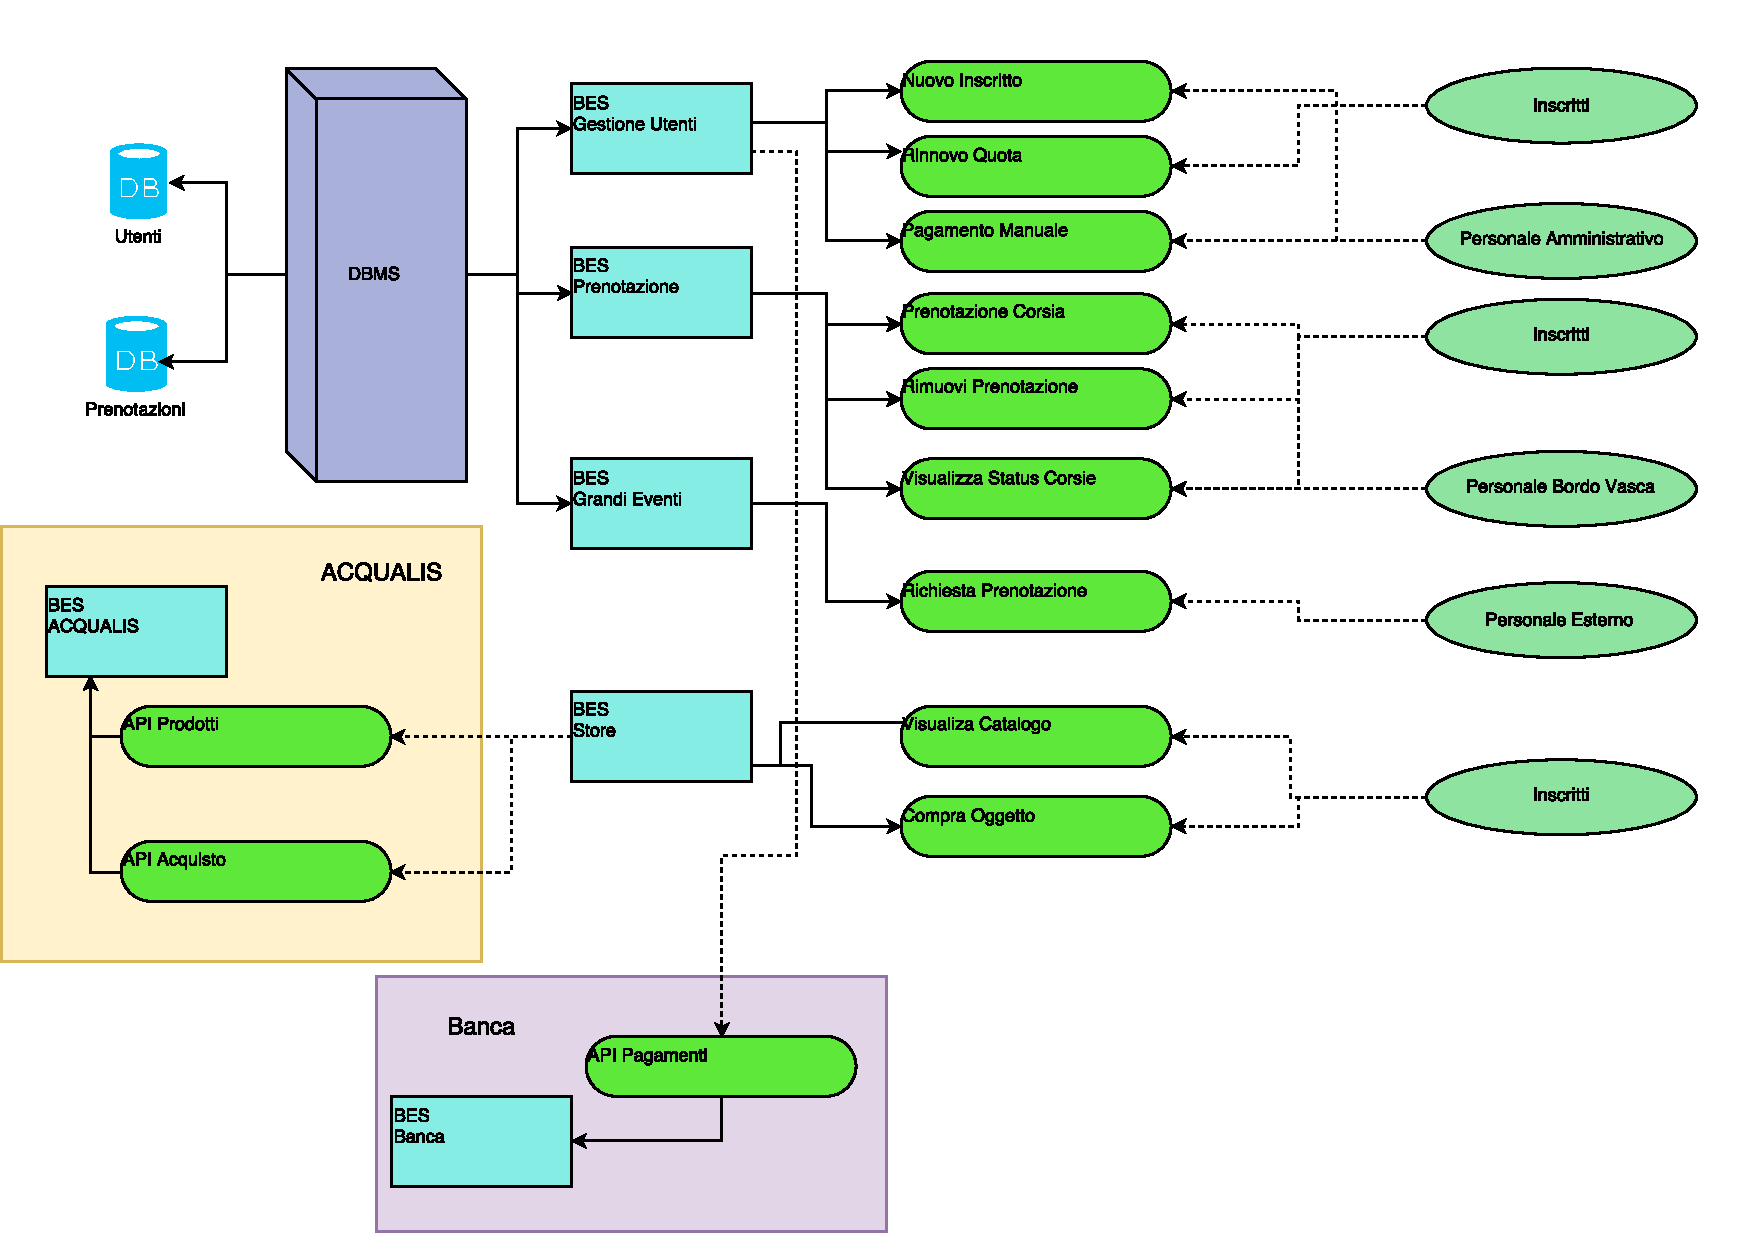
\includepdf[landscape=true]{Party.pdf}

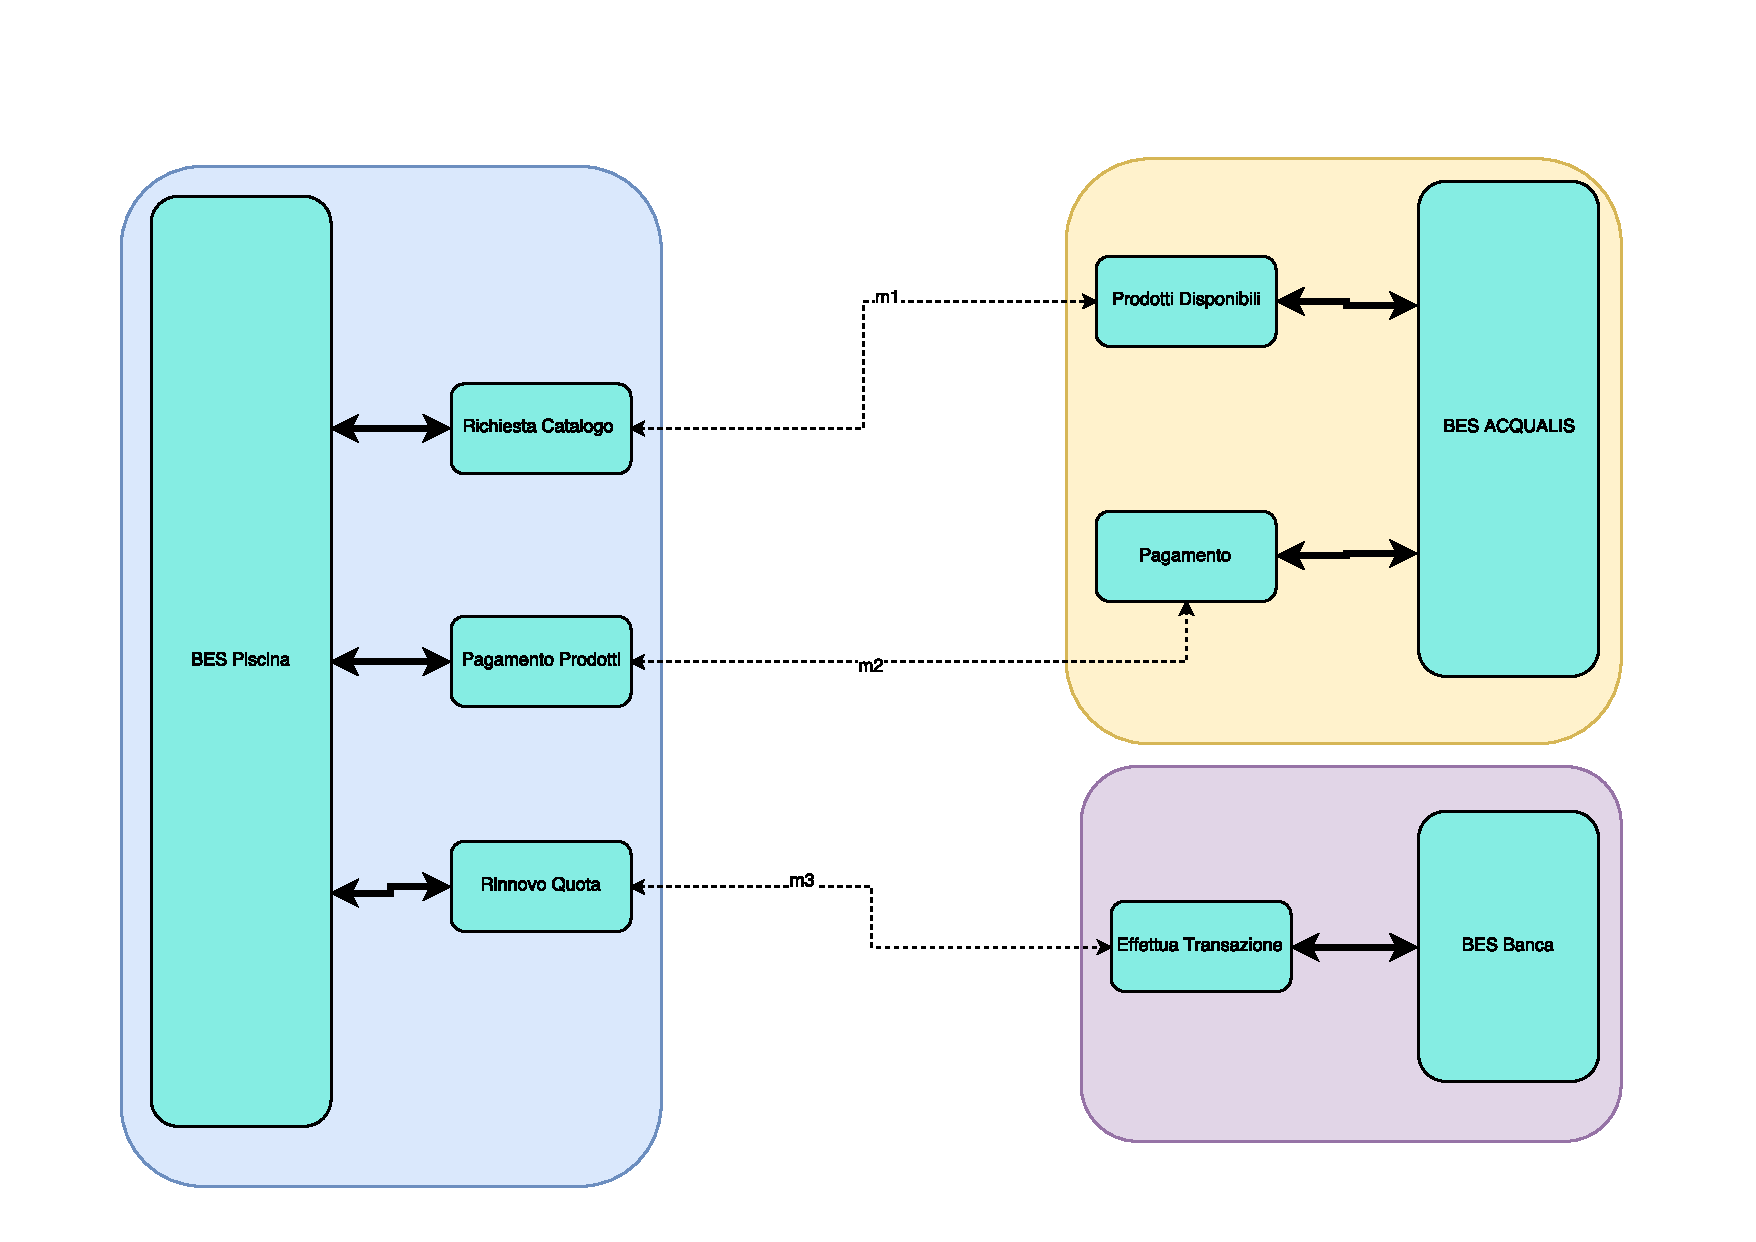
\includepdf[landscape=true]{Market.pdf}

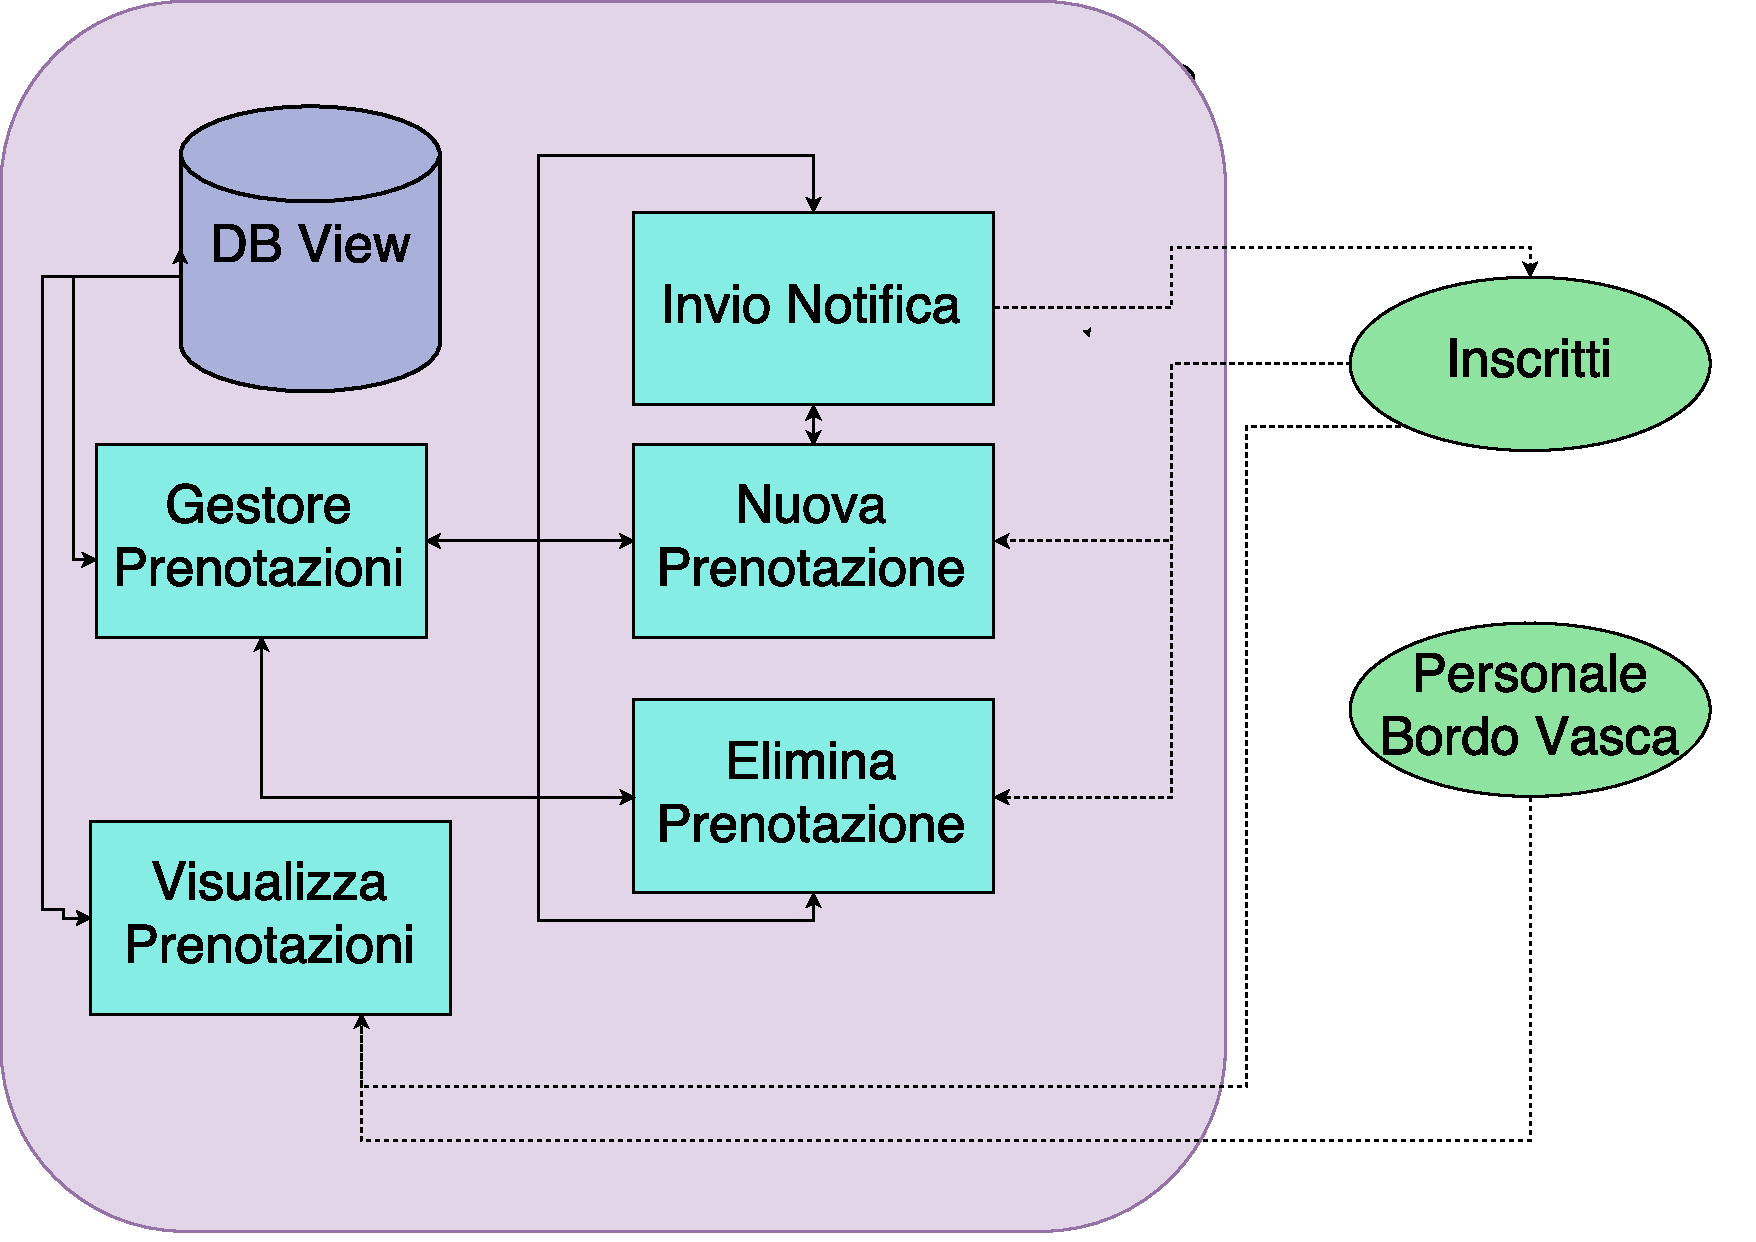
\includepdf[landscape=true]{System.pdf}

\end{document}
